\documentclass{beamer}
\usepackage[utf8]{inputenc}
\usepackage{amsfonts,amsmath,oldgerm}
\usetheme{sintef}

\usefonttheme[onlymath]{serif}

\titlebackground*{assets/background}

\newcommand{\hrefcol}[2]{\textcolor{cyan}{\href{#1}{#2}}}

\title{Riconoscimento di dispositivi di
protezione individuale in ambito
industriale tramite infrastruttura
cloud}
\subtitle{\tiny Compilato in \LaTeX}
\course{Corso di Laurea Magistrale in Ingegneria Informatica}
\author{ \href{mailto:rei.zoto@studenti.polito.it}{}\\{\small Rei Zoto \hspace{1cm} Relatore: Prof. Luca Ardito}
}
\begin{document}
\maketitle

\section{Introduzione}

\begin{frame}{Infortuni sul Lavoro}
\begin{itemize}
    \item Problemi
    	\begin{itemize}
    		\item costi diretti
    		\item costi indiretti
    		\item impatto sulla società
    	\end{itemize}	
    \item Soluzioni
    \begin{itemize}
    	\item Prevenzione: valutazione dei rischi, idoneità del lavoratore, formazione
    	\item Dispositivi di sicurezza individuale (DPI)
    	\item Sistemi automatici al posto di controlli manuali
    \end{itemize}
\end{itemize}
\end{frame}
\begin{frame}{INAIL: Statistiche sugli infortuni}
  \begin{itemize}
  		\item Totale infortuni nella manifattura anno 2022: 13,9\%
  \end{itemize}  	  
  \begin{columns}
    % Prima colonna
    \begin{column}{0.4\textwidth}
      \centering
      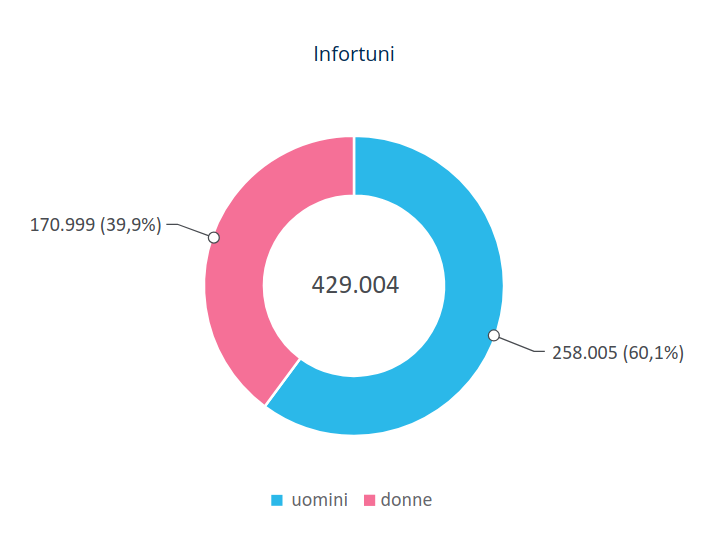
\includegraphics[width=\textwidth]{images/totaleinfortuni.png}
      \vspace{2mm}
      \small{Totale infortuni divisi per genere}
    \end{column}
    % Seconda colonna
    \begin{column}{0.25\textwidth}
      \centering
      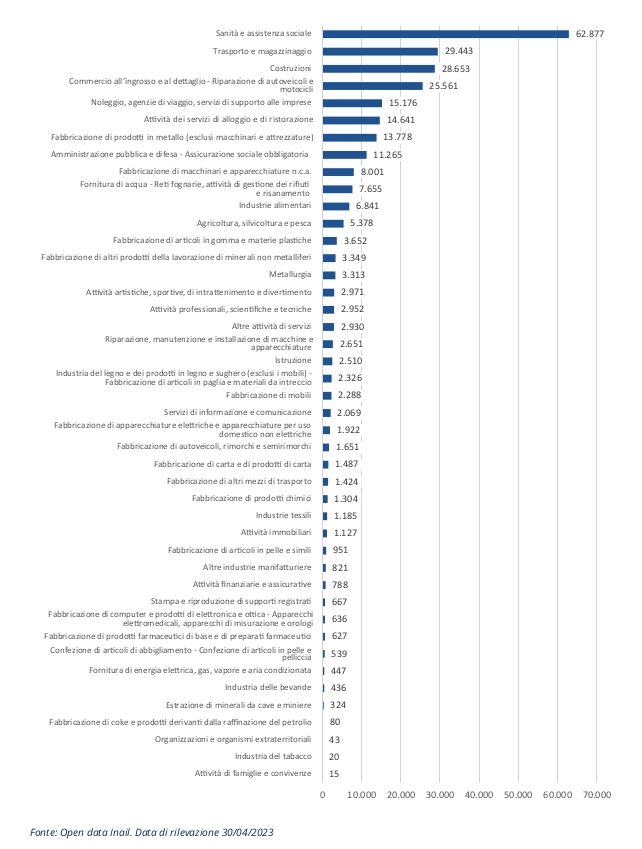
\includegraphics[width=\textwidth]{images/infortuni_industria_e_servizi.png}
      \vspace{2mm}
      \small{Infortuni per categoria}
    \end{column}
  \end{columns}
\end{frame}











\begin{frame}{OSHA-EU: Impatto sulla produttività nazionale}

  \begin{columns}  
    % Prima colonna
    \begin{column}{0.5\textwidth}
      \begin{itemize}
%  	\item DALY: stima anni di vita persi per infortuni e malattie
%	\item VSLY: metodologia che associa agli anni di vita un valore monetario
	\item bottom-up: totale infortuni 6,3\% su PIL
	\item top-down (VSLY): mediana infortuni 7,7\% sul PIL	
	\item Effetti dominio industriale sul PIL italiano 20MLD (1\%)
  \end{itemize}
      \centering
      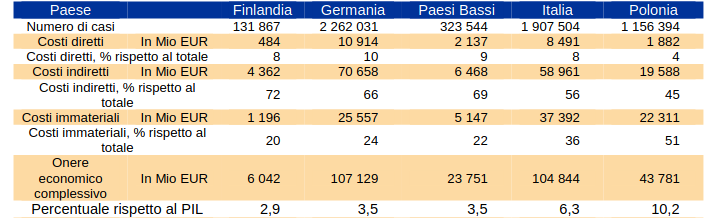
\includegraphics[width=\textwidth]{images/onere_infortuni_ba.png}
      \vspace{2mm}
      \small{Approccio bottom-up}
    \end{column}

    % Seconda colonna
    \begin{column}{0.5\textwidth}
      \centering
      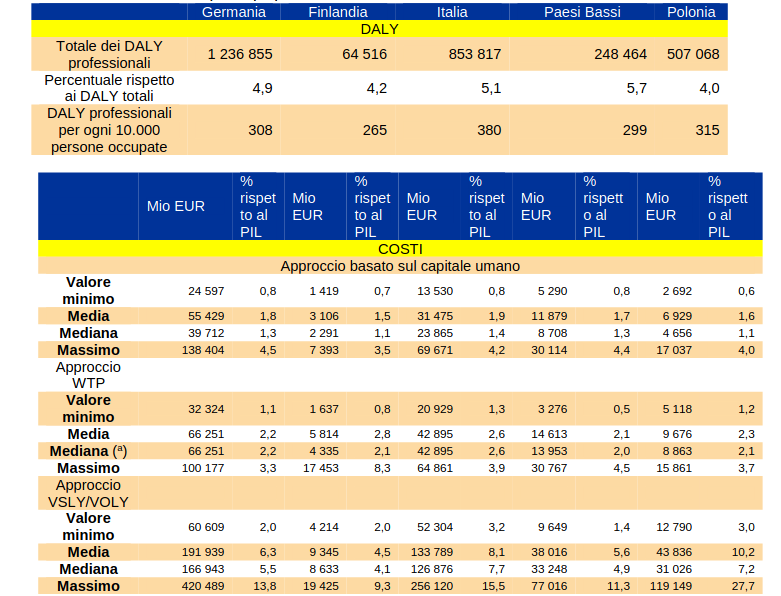
\includegraphics[width=\textwidth]{images/onere_infortuni_td.png}
      \vspace{2mm}
      \small{Approccio top-down}
    \end{column}
  \end{columns}
\end{frame}

\begin{frame}{Obiettivi e Motivazioni}
\textbf{Scopo del lavoro}:
\begin{itemize}
\vspace{0.2cm}
	\item Implementazione di un sistema integrato con il cloud per la rilevazione di dispositivi di sicurezza    
\end{itemize}
\vspace{0.3cm}
\textbf{Motivazioni personali}:
\begin{itemize}
    \item Interesse sistemi IoT e deep learning
    \item Scelta della tesi durante lo studio di sistemi operativi, virtualizzazione ed estensione dei concetti al cloud.
\end{itemize}
\end{frame}







\section{Panoramica}

\begin{frame}{Innovazione nell'industria: fattori abilitanti}
\begin{itemize}
	\item Quantità di dati disponibili grazie dispositivi connessi alla rete
	\item Avanzamenti Deep Learning
	\item Cloud Computing: potenza di calcolo ed integrazione di modelli e dati nell'ecosistema industriale
	\item Investimenti %https://www.grandviewresearch.com/industry-analysis/industrial-internet-of-things-iiot-market
\end{itemize}
\end{frame}

%prova a rendere più densa questa slide
\begin{frame}{Computer Vision}
  \begin{columns}[T,onlytextwidth]
    \begin{column}{0.55\textwidth}
      \begin{itemize}
      	\vspace{0.5cm}        
        \item Utilizzo di modelli di deep learning per diversi task di computer vision
        \vspace{0.3cm}
          % classificazione, object detection, image segmentation, ...
        \item Dominio di applicazione: Object Detection
        \vspace{0.3cm}
        \item Modello utilizzato: Amazon Rekognition      
      \end{itemize}
    \end{column}

    \begin{column}{0.4\textwidth}
      \centering
      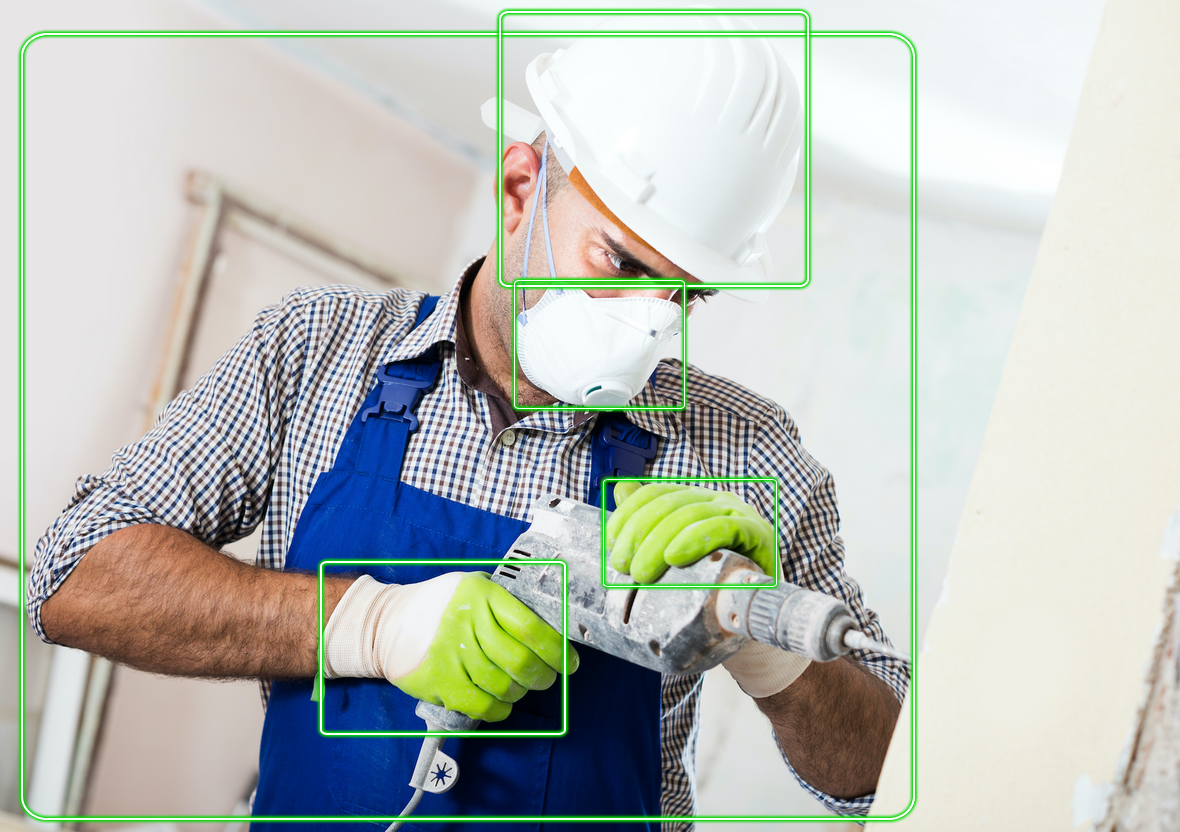
\includegraphics[width=\textwidth]{images/worker-with-bb.png}
    \end{column}
  \end{columns}
\end{frame}

\begin{frame}{Lavori Correlati}
  \begin{columns}
    % Prima colonna
    \begin{column}{0.5\textwidth}
      \centering
      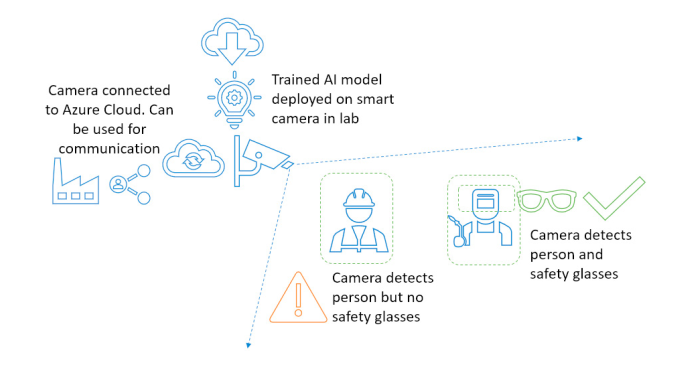
\includegraphics[width=\textwidth]{images/relw1-system.png}
      \tiny B. Balakreshnan and Others, “Ppe compliance detection using artificial
intelligence in learning factories”
    \end{column}

    % Seconda colonna
    \begin{column}{0.5\textwidth}
      \begin{figure}
      \centering
      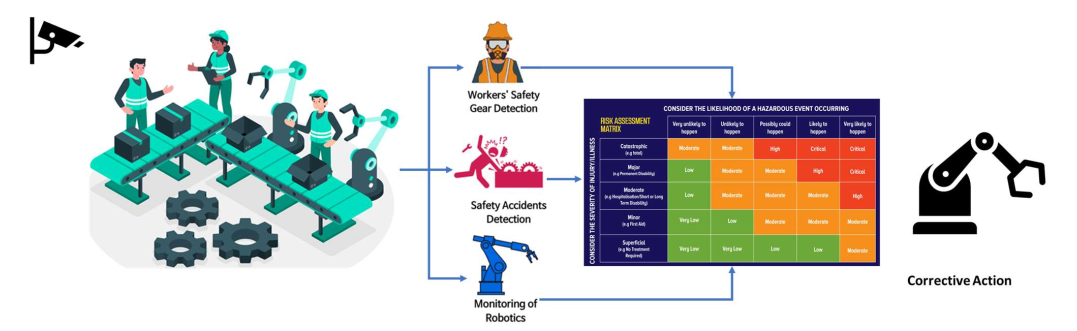
\includegraphics[width=\textwidth]{images/safety-system.png}
      \tiny {I. Yousif and Others, “Safety 4.0: Harnessing computer vision for
advanced industrial protection”}
	\end{figure} 
    \end{column}
  \end{columns}
\end{frame}

%\begin{frame}{Lavori Simili (cont.)}
%  \begin{columns}
    % Prima colonna
%    \begin{column}{0.4\textwidth}
%      \centering
%      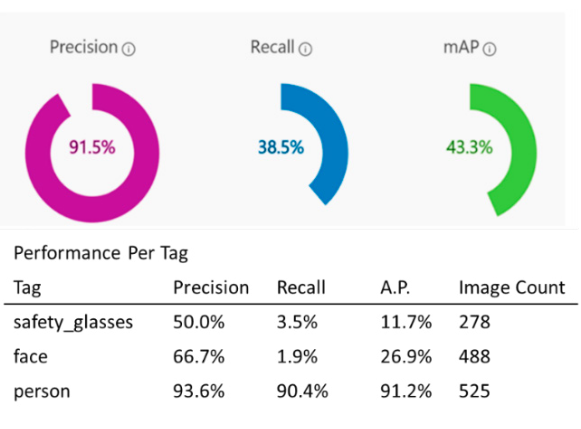
\includegraphics[width=\textwidth]{images/relw1.png}
%      \vspace{2mm}
%      \small{1) Metriche sulle classi maschera protettiva, volti e persone}
%    \end{column}

    % Seconda colonna
%    \begin{column}{0.4\textwidth}
%      \centering
%      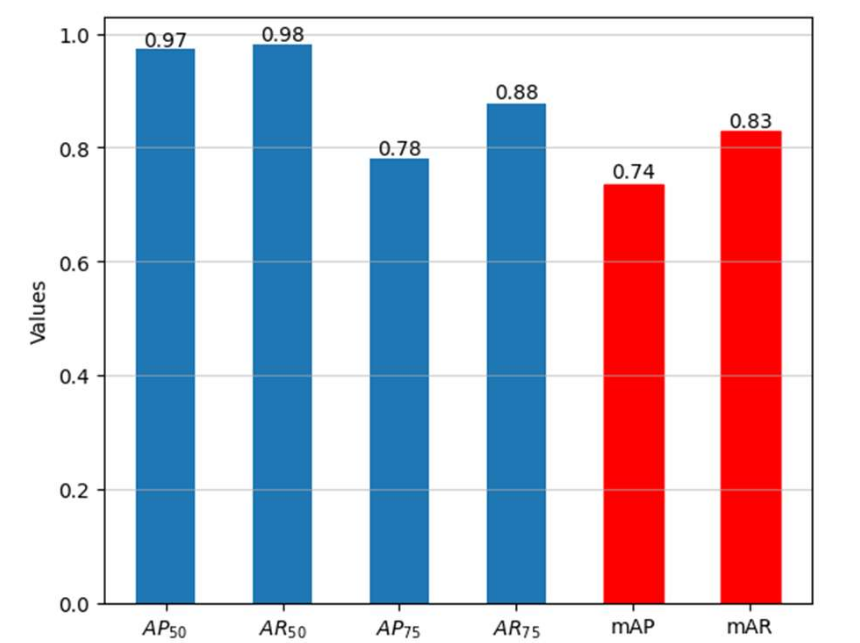
\includegraphics[width=\textwidth]{images/safety-system-results.png}
%      \vspace{2mm}
%      \small{2) Mean Average Precision sulle classi casco e giubotto protettivo}
%    \end{column}
%  \end{columns}
%\end{frame}


\begin{frame}{Soluzione}

\begin{itemize}
    \item Entry-level
    \begin{itemize}
        \item Mostrare quali sono le possibilità con l'integrazione dei diversi fattori discussi.
        \item Approccio che supera barriere di ingresso per piccole aziende sia nei tempi che nei costi.
    \end{itemize}
    
    \item Risposta al problema con un sistema near real-time.

    \item Motivazioni:
    \begin{itemize}
        \item Mancanza di benchmark specifici per dispositivi di sicurezza.
        \item L'approccio near real-time è conservativo
        \begin{itemize}
            \item Tempi di risposta del modello non veloci (servizio pensato per tutti gli utenti AWS, tipicamente 5 fps).
            \item Latenza intrinseca per la comunicazione con il cloud e problemi di connettività.
        \end{itemize}
    \end{itemize}
\end{itemize}

\end{frame}

\begin{frame}{Tecnologie, protocolli e servizi}
    \centering
    \begin{tabular}{ccc}
        % Prima Riga: Docker, AWS, Apache Flink
        
\includegraphics[width=0.2\textwidth]{images/docker_logo.png} & 
        
\includegraphics[width=0.2\textwidth]{images/aws_logo.png} & 
        
\includegraphics[width=0.2\textwidth]{images/apache_flink_logo.jpeg} \\
         	& 	 & Apache Flink \\
        \vspace{0.5cm} \\ % Spazio aggiuntivo tra le righe
        % Seconda Riga: MQTT, RTSP, Publish/Subscribe
        
\includegraphics[width=0.2\textwidth]{images/mqtt_logo.png} & 
        
\includegraphics[width=0.2\textwidth]{images/rtsp_logo.png} \\ 
    \end{tabular}
    \footlinecolor{sintefyellow}
\end{frame}

%vedi se aggiungere, forse too much ma sarebbe utile per la comprensione
%\begin{frame}{Servizi utilizzati}
%\end{frame}
\section{Implementazione}
\begin{frame}{Use Case}
\begin{columns}
\begin{column}{0.5\textwidth}
\footnotesize
\begin{itemize}
	\item Scenario	
\begin{itemize}
\footnotesize
	\item Uno o più impiegati entrano all’interno di una certa area di sicurezza e si trovano in prossimità di un macchinario attivo
	\item Una telecamera sul soffitto ed una frontale monitorano l’area di sicurezza
	\item La zona è definita da un insieme di ancore dotate di sensori che rilevano i tag indossati dai lavoratori. 
\end{itemize}
	\item Il sistema genera allarme e spegne il macchinario se tutti gli operatori	
\begin{itemize}
\footnotesize
	\item non possiedono i dispositivi di sicurezza
	\item non sono abilitati ad agire sulla macchina
\end{itemize}
\end{itemize}
\end{column}
\begin{column}{0.5\textwidth}
	\begin{figure}	
	\centering
    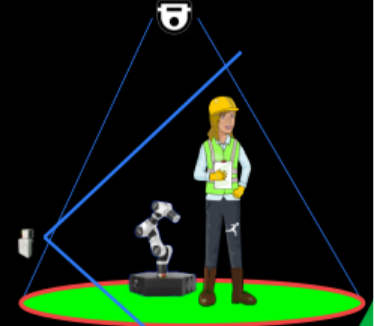
\includegraphics[width=0.7\textwidth]{images/use-case.png}
    \end{figure}
\end{column}
\end{columns}
\end{frame}

\begin{frame}{Architettura}
\begin{figure}
    \centering
    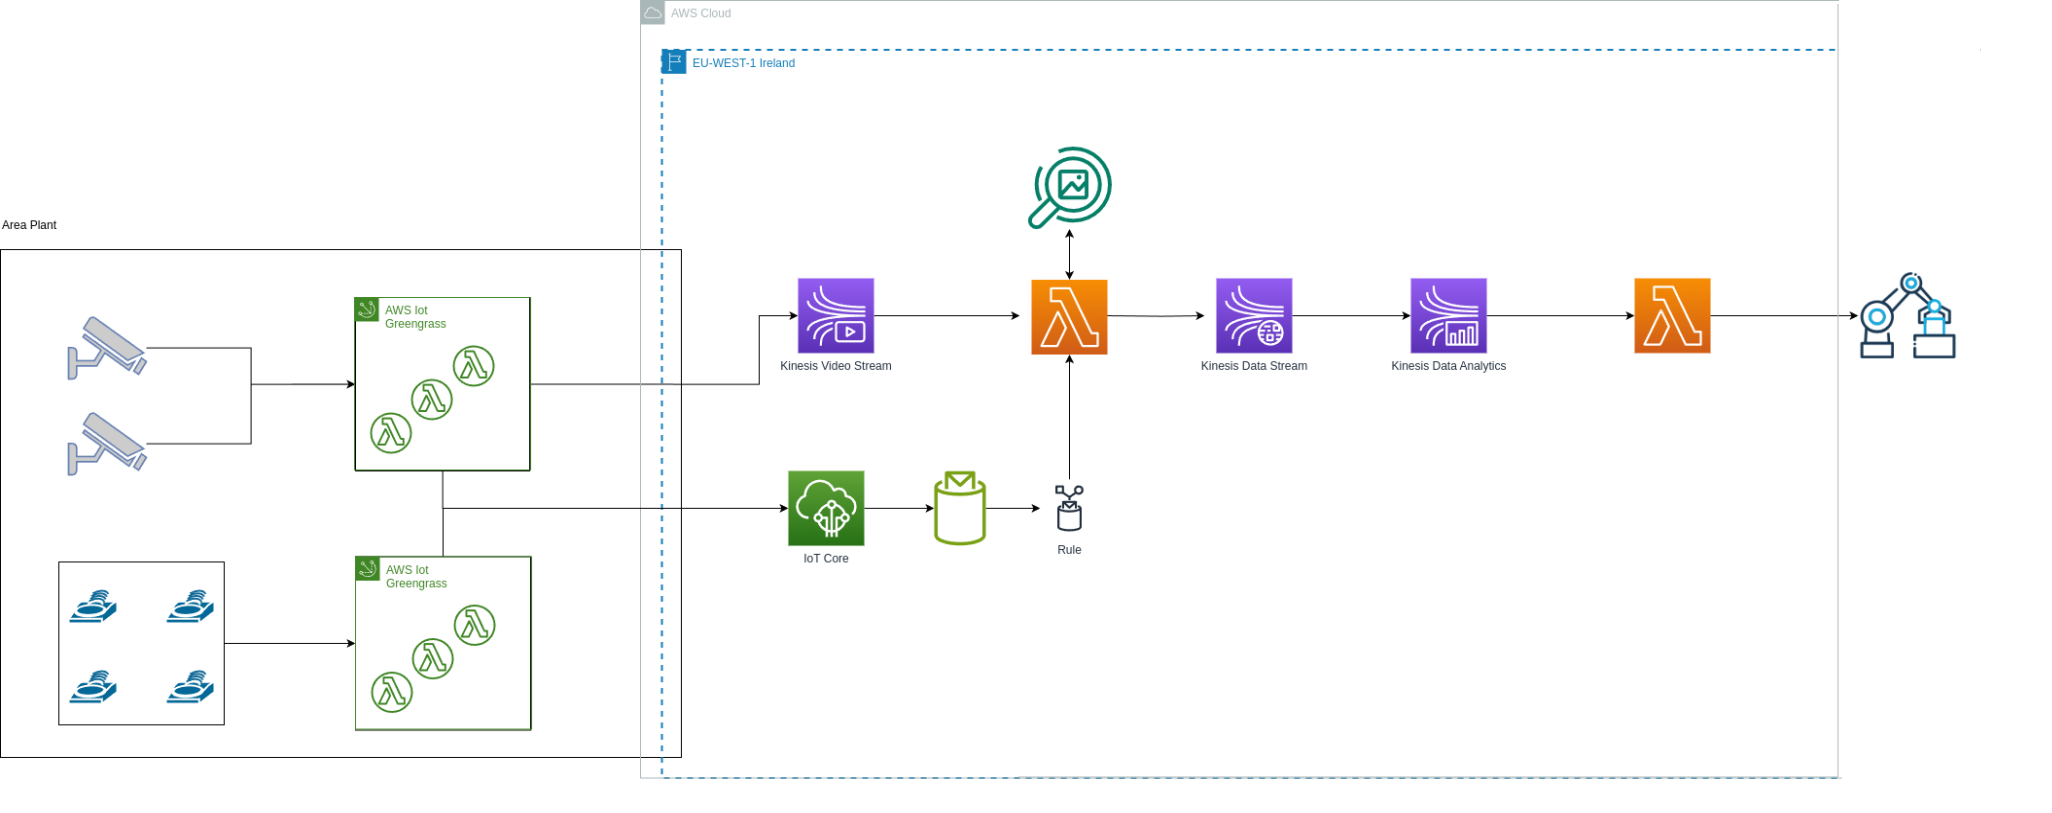
\includegraphics[width=0.9\textwidth]{images/architettura.png}
%    \caption{Diagramma dell'Architettura Generale}
\end{figure}
\end{frame}

%\begin{frame}{Ingestion e Preprocessing}
%\begin{figure}
%    \centering
%    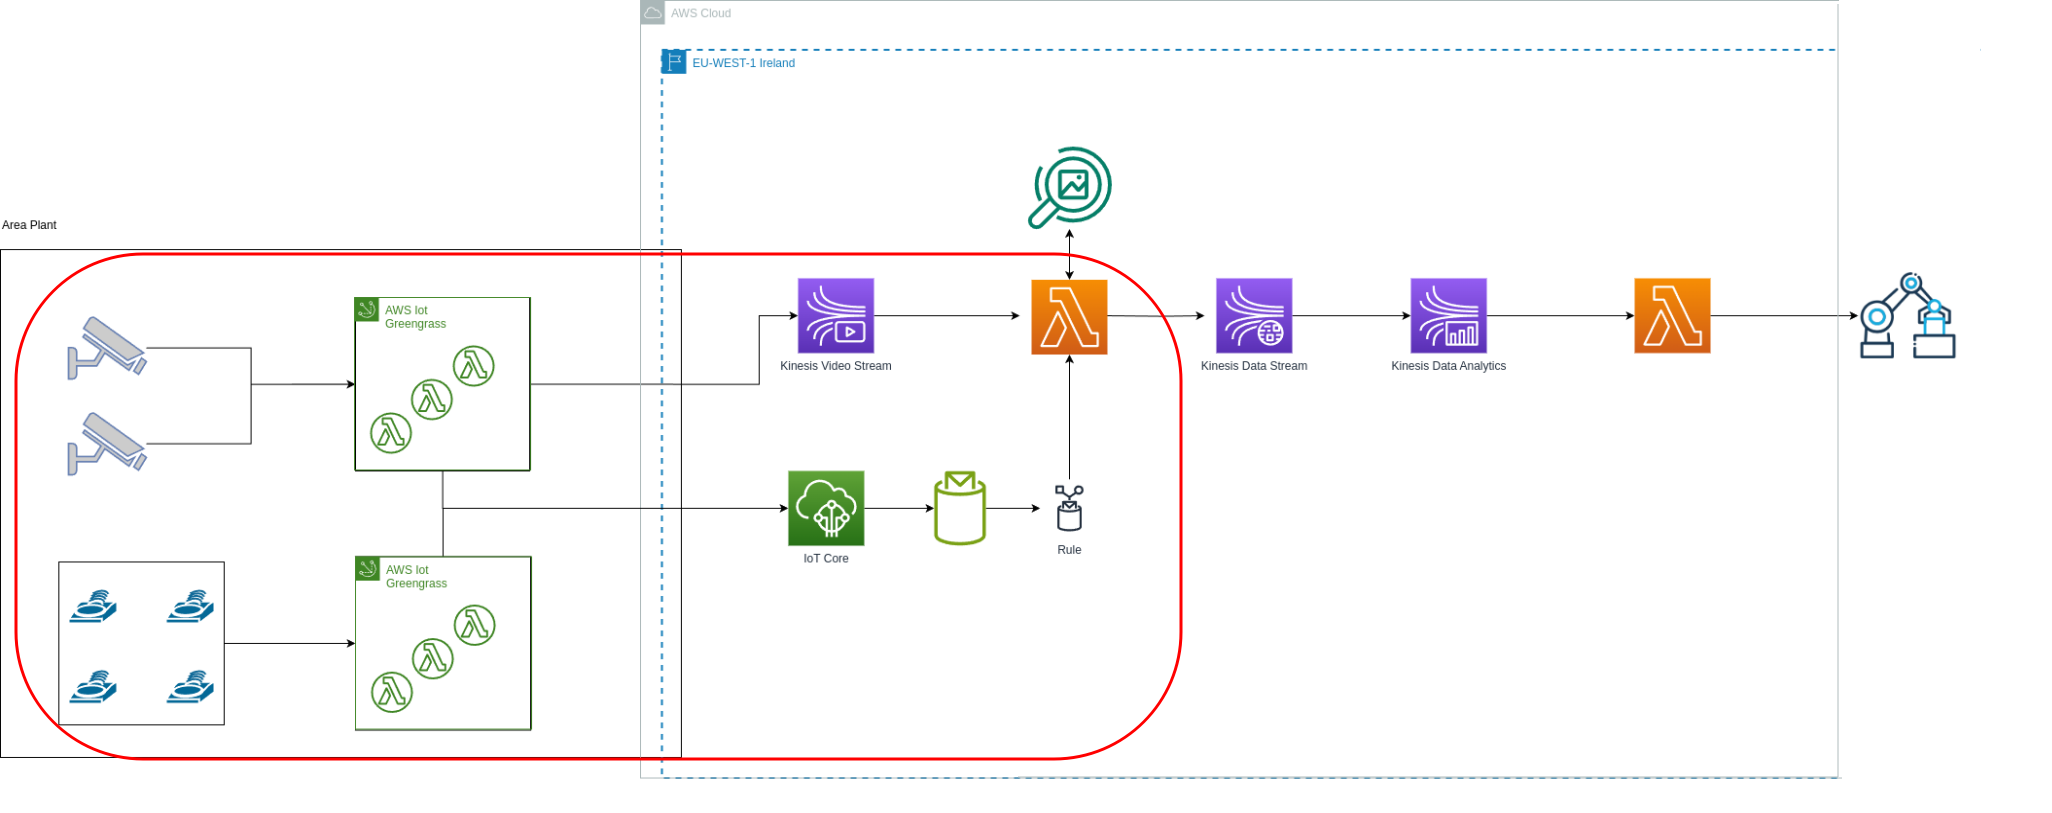
\includegraphics[width=0.9\textwidth]{images/sottosistema-ingestion.png}
%    \caption{Diagramma dell'Architettura Generale}
%\end{figure}

%\end{frame}

%\begin{frame}{Big Data Processing}
%\begin{figure}
%    \centering
%    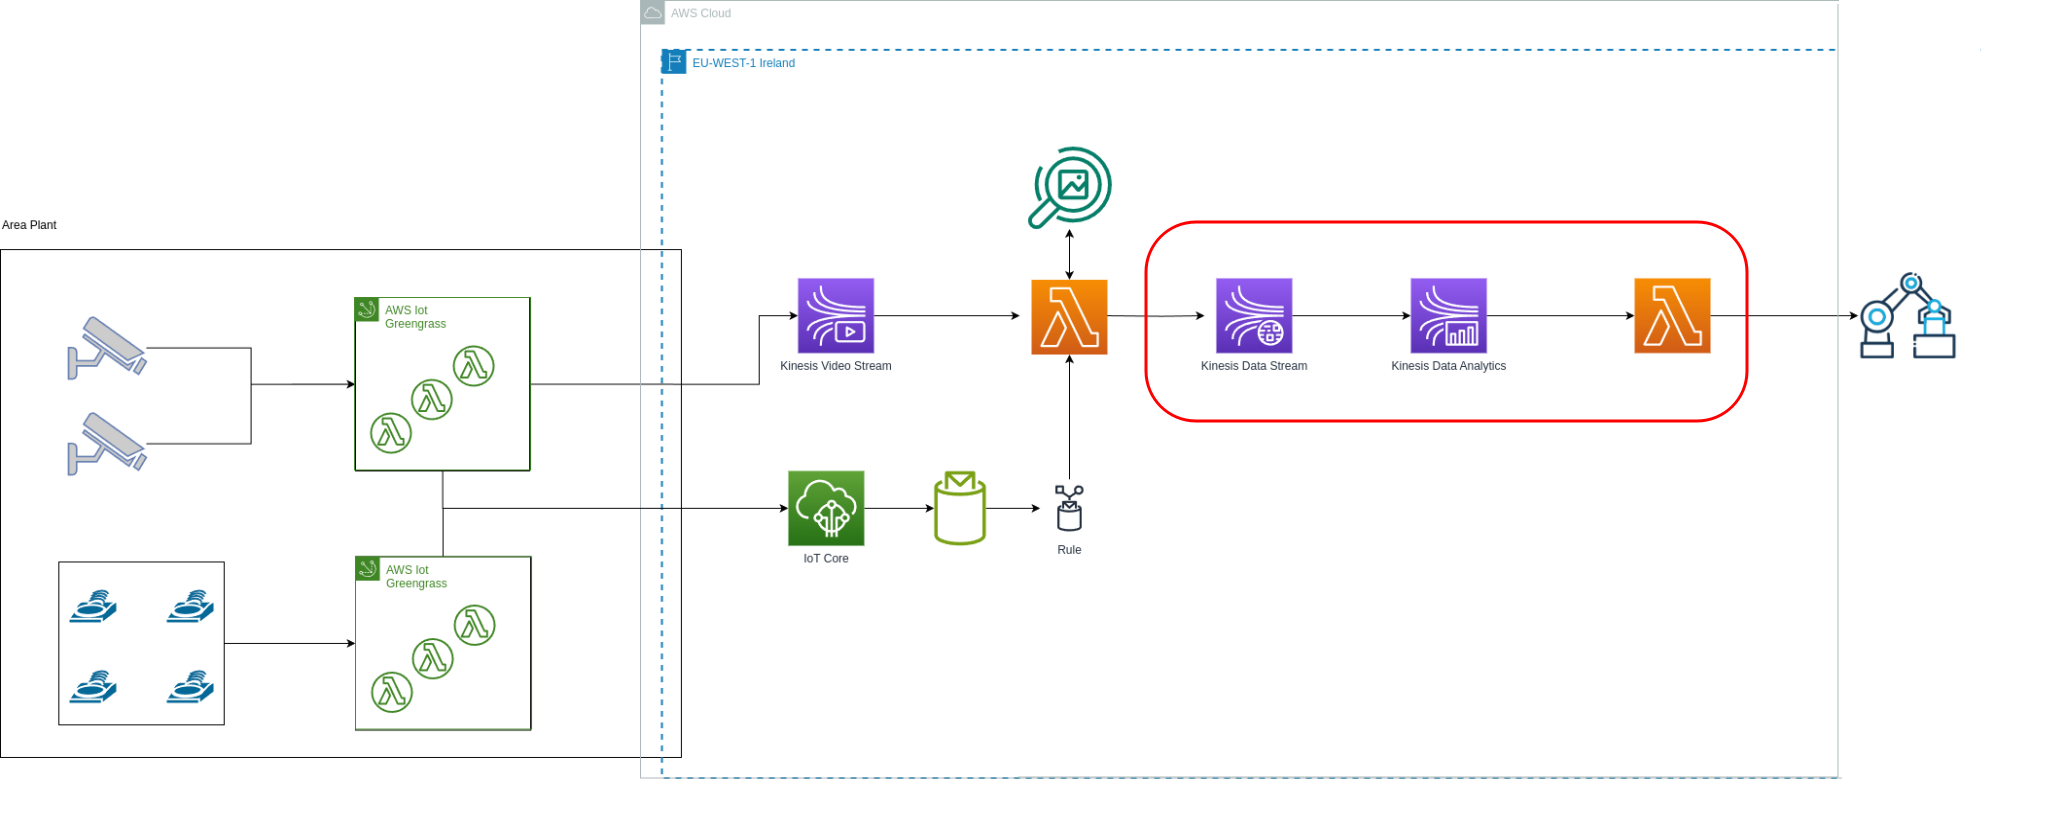
\includegraphics[width=0.9\textwidth]{images/processing-subsystem.png}
%    \caption{Diagramma dell'Architettura Generale}
%\end{figure}

%\end{frame}


\section{Risultati}

\begin{frame}{Test case}

\begin{itemize}
    \item Rilevazioni dirette dal video feed effettuate per la classe casco protettivo
    \item machine state: TRUE
\end{itemize}
\vspace{0.5cm}

\begin{table}[h]
\centering
\begin{tabular}{c c c c c}
\hline
\textbf{tags} & \textbf{people} & \textbf{equipment} & \textbf{expected result} \\
\hline
0 & 1 & TRUE & ALARM \\
1 & 1 & FALSE & ALARM \\
0 & 1 & FALSE  & ALARM \\
2 & 2 & TRUE;FALSE & ALARM \\
1 & 2 & TRUE;FALSE & ALARM \\
\hline
\end{tabular}
\end{table}

%\vspace{0.5cm}
%\textit{\footnotesize (Le etichette dei parametri verranno spiegate oralmente.)}
\end{frame}


\begin{frame}{Metriche}
\begin{itemize}
    \item Rilevazione del casco corretta in quasi tutti i test:
        \begin{itemize}
            \item In un caso rilevazione presente nell’80\% dei frame (soglia accettata: 70\%)
            \item Nelle altre prove, nessuna rilevazione poiché il casco non era indossato
        \end{itemize}
    \item Conteggio delle persone sempre esatto e matching corretto su tutti i frame
    \item Regole per l’attivazione dell’allarme sempre soddisfatte
    \item Tempi di risposta near real-time:
        \begin{itemize}
            \item Ritardo totale medio (dall’evento al ritorno dell’analisi) circa 2,56 s (deviazione standard: 0,374 s)
            \item Ritardo singolo servizio (Rekognition): ~850 ms
            \item Ritardo big data application: ~550 ms
        \end{itemize}
\end{itemize}
\end{frame}

\begin{frame}{Limitazioni}
\begin{itemize}
    \item Prove non eseguite in un ambiente industriale reale
    \item Insieme dei test non automatizzato: implementazione manuale di script e parametrizzazione
    \item Amazon Rekognition: impossibilità di installare il modello sull'edge
    \item Utilizzo di due sole telecamere, scalabilità del sistema non verificata
    \item Potenza insufficiente del gateway per gestire un elevato numero di dispositivi e flussi video RTSP
\end{itemize}
\end{frame}

\section{Conclusioni}

\begin{frame}{Conclusioni}
\begin{itemize}
    \item Obiettivi raggiunti
	\begin{itemize}
		\item  Generazione infrastruttura cloud e funzionalità quasi in tempo reale 
    	\item Capacità di identificare persone autorizzate e dotate di dispositivi di sicurezza
    \item Architettura facilmente replicabile con utilizzo Infrastructure as Code (IaC)
    \end{itemize}
    \item Soluzione già utilizzabile come punto di partenza, pur non essendo confrontabile con lavori edge-based.
\end{itemize}
\end{frame}

\begin{frame}{Sviluppi Futuri}
\begin{itemize}
    \item Creazione di un modello custom e deploy sull’edge per ridurre latenza e dipendenza dal cloud.
    \item Integrazione con robot tramite container ROS e AWS Greengrass per favorire comunicazione e controllo locale.
    \item Automazione dell’ambiente di test con orchestratori (ad es. Step Functions) e CI/CD (CodePipeline).
    \item Adattabilità del sistema a contesti variabili, con aggiornamenti dinamici delle soglie (Apache Flink + DynamoDB).
    \item Estensione del logging (CloudWatch) e generazione di metriche e statistiche consultabili via interfaccia utente.
\end{itemize}
\end{frame}


\section*{Domande}

\backmatter
\end{document}
